\documentclass[12pt]{report}

%Vous souciez pas de tout les packages, j'ai oublié ce que fait la moitié d'entre eux

\usepackage[utf8]{inputenc}
\usepackage[T1]{fontenc}
\usepackage[francais]{babel}
%\usepackage{layout}
\usepackage[left=3cm,right=3cm,top=3cm,bottom=3cm]{geometry}
%\usepackage{setspace}
\usepackage{soul}
\usepackage[normalem]{ulem}
%\usepackage{eurosym}
%\usepackage{bookman}
%\usepackage{charter}
%\usepackage{newcent}
%\usepackage{lmodern}
%\usepackage{mathpazo}
%\usepackage{mathptmx}
%\usepackage{url}
%\usepackage{verbatim}
%\usepackage{moreverb}
%\usepackage{listings}
%\usepackage{fancyhdr}
%\usepackage{wrapfig}
\usepackage{color}
%\usepackage{colortbl}
\usepackage{amsmath}
\usepackage{amssymb}
\usepackage{mathrsfs}
%\usepackage{asmthm}
%\usepackage{makeidx}
\usepackage{graphicx}
\usepackage{tabularx}
\usepackage{tgtermes}
\usepackage{titlesec}
\usepackage[final]{pdfpages} 
\usepackage{epsfig}
\usepackage{comment}
\usepackage{float}
\usepackage{amsmath}
\renewcommand{\emph}{\textit}
\renewcommand{\thesection}{\arabic{section}}
\renewcommand{\thesubsection}{\arabic{section}.\arabic{subsection}}
\titleformat*{\subsection}{\bfseries}
\parskip=5pt

%Information pour la page de garde

\title{TP 2 - La transformée en cosinus discrète 2D}
\author{Guillaume \bsc{Versal}, Jean-Baptiste \bsc{Morice}}
\date{\today}


\begin{document}



%Commande qui crée la page de garde
\maketitle

\tableofcontents

\newpage
\section*{Introduction}

Ce TP a pour objectif :
\begin{itemize}
\item la prise en main de la transformée en cosinus discrète 2D sur des images naturelles ;
\item l'implémentation d'une transformée par bloc 8x8.\\
\end{itemize}
Pour ce TP nous disposions d'une image de base, "boats.pgm", représentant des bateaux amarés dans un port. Cette image est intéressante pour observer les effets de la transformée en cosinus car elle présente des détails fins au niveau de la mâture du bateau sur lesquels les éventuels artefacts de compression seront plus visibles.


\newpage
\section{Notre travail}

\subsection{DCT et DCT inverse}
Dans un premier temps nous devions mettre en place un programme qui convertit une image encodée sur trois canaux en BGR vers YCrCb, puis qui appliquer la DCT sur chacune de ces composantes. Pour vérifier la réversibilité du processus nous devions appliquer la DCT inverse sur le résultat obtenu et comparer l'EQM et le PSNR de l'image finale obtenue et de l'image originale.\\

L'image originale suivante :

%Image originale
\begin{figure}[H]
\begin{center}
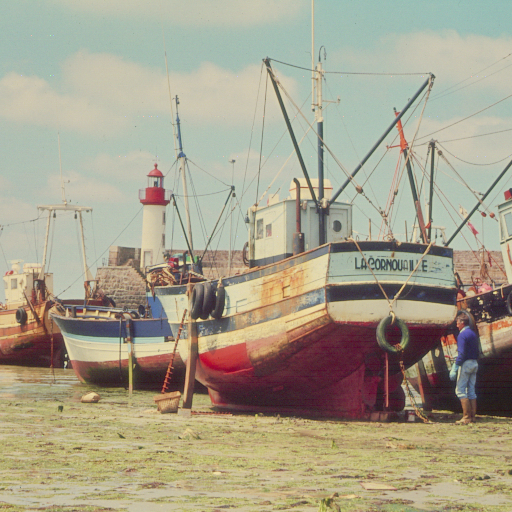
\includegraphics[scale=0.5]{../boats.jpg} 
\caption{Image originale}
\end{center}
\end{figure}

Dont les histgorammes des canaux YCrCb sont :

\begin{figure}[H]
\begin{center}
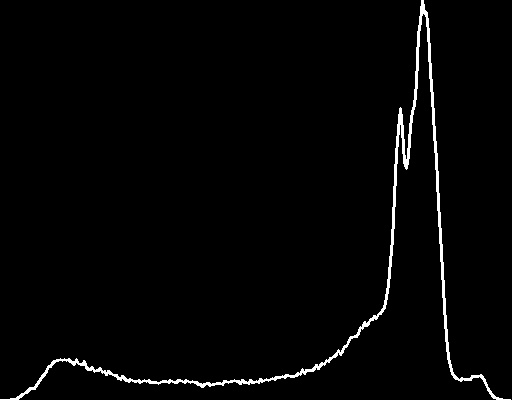
\includegraphics[scale=0.25]{../ImageRes/orig_histo_0.jpg} 
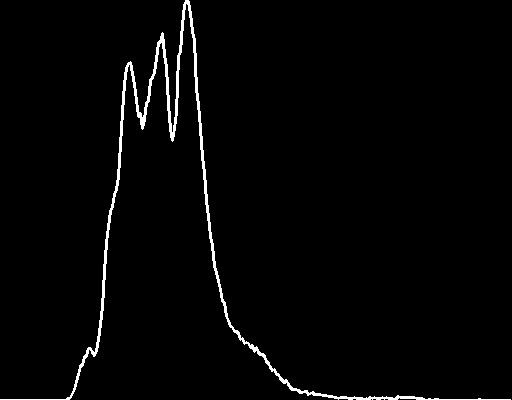
\includegraphics[scale=0.25]{../ImageRes/orig_histo_1.jpg} 
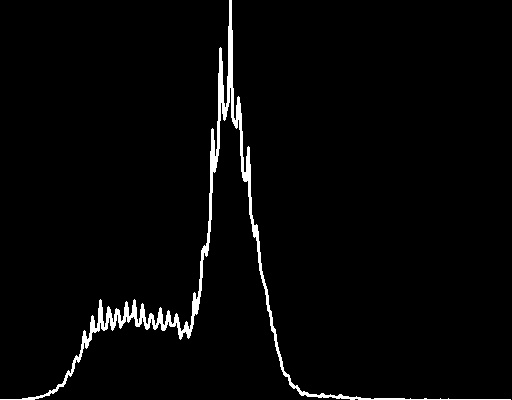
\includegraphics[scale=0.25]{../ImageRes/orig_histo_2.jpg} 
\caption{Histogrammes des canaux Y, Cb et Cr de l'image "boats.pgm"}
\end{center}
\end{figure}

\begin{itemize}
\item Entropie canal Y : 6.64908
\item Entropie canal Cr : 4.61065
\item Entropie canal Cb : 4.87461
\end{itemize}

Donne donc le résultat suivant :

%Image originale
\begin{figure}[H]
\begin{center}
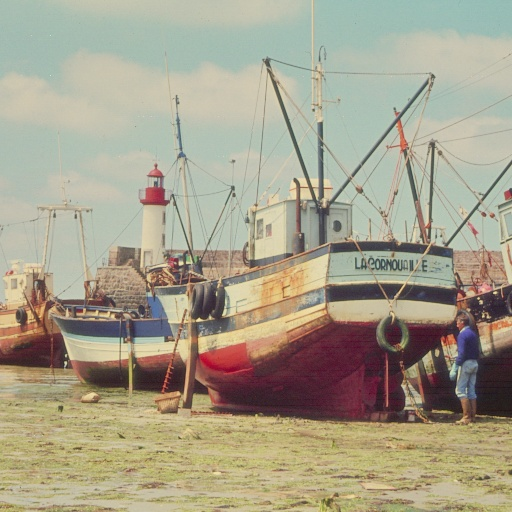
\includegraphics[scale=0.5]{../ImageRes/idct_result.jpg} 
\caption{Résultat de la DCT inverse}
\end{center}
\end{figure}

L'EQM entre ces deux images vaut 0 et le PSNR est infini, ce qui confirme le bon fonctionnement de la transformée et de la transformée inverse.

\subsection{Répartition des coefficients DCT}
Dans un second temps nous souhaitions visualiser ces coefficients. Pour les rendre visuellement interprétables nous leur avons appliqué un compression logarithmique ainsi qu'une color map.\\

Pour l'image "boats.pgm" nous obtenons les résultats suivants :

\begin{figure}[H]
\begin{center}
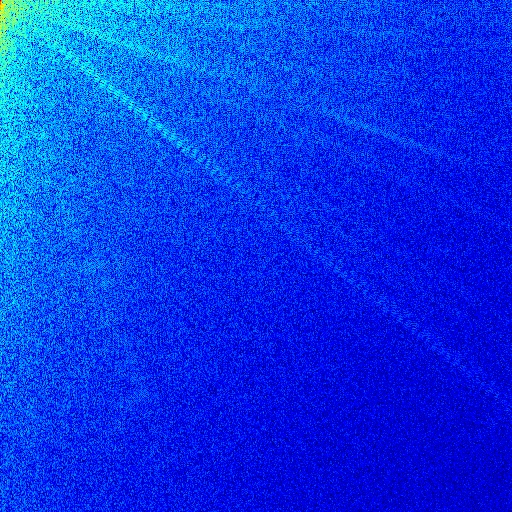
\includegraphics[scale=0.25]{../ImageRes/dct_0.jpg} 
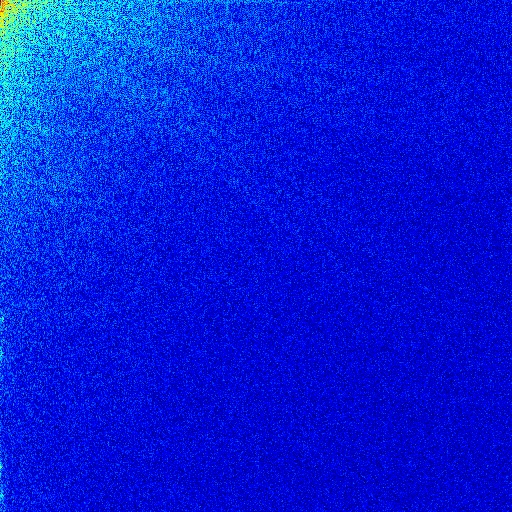
\includegraphics[scale=0.25]{../ImageRes/dct_1.jpg} 
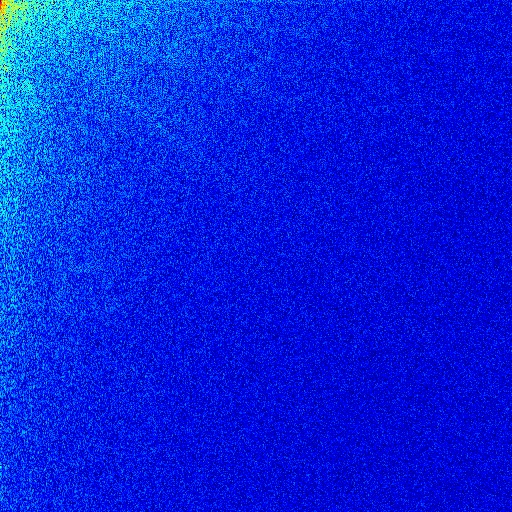
\includegraphics[scale=0.25]{../ImageRes/dct_2.jpg} 
\caption{Coefficients DCT pour les canaux Y, Cb et Cr de l'image "boats.pgm"}
\end{center}
\end{figure}

Observons les histogrammes de ces images :

\begin{figure}[H]
\begin{center}

\includegraphics[scale=0.25]{../ImageRes/dct_histo_0.jpg} 

\includegraphics[scale=0.25]{../ImageRes/dct_histo_1.jpg} 
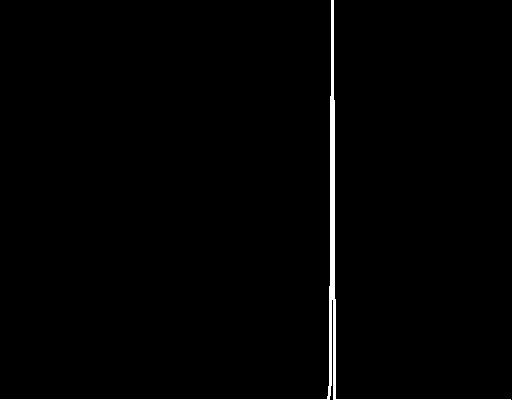
\includegraphics[scale=0.25]{../ImageRes/dct_histo_2.jpg} 
\caption{Histogrammes des coefficients DCT pour les canaux Y, Cb et Cr de l'image "boats.pgm"}
\end{center}
\end{figure}

Les valeurs des coefficients DCT du canal Y ont pour entropie 4.56095, ceux du canal Cr 2.54804, et ceux du canal Cb 2.79877.

Comparer les histogrammes 

\subsection{Influence des coefficients DCT sur la qualité de l'image}

\subsubsection{Premier masquage : coin bas droit}

\begin{figure}[H]
\begin{center}
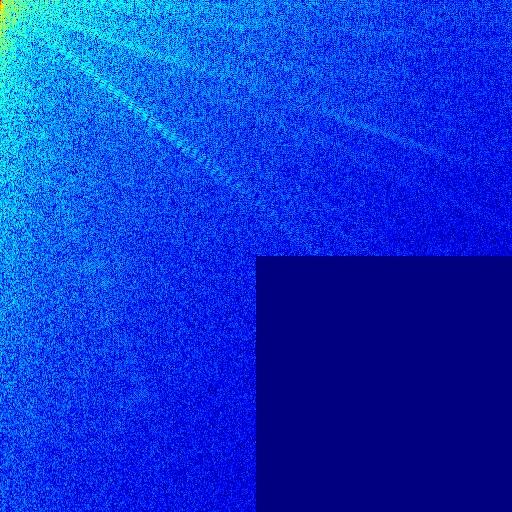
\includegraphics[scale=0.25]{../ImageRes/dct_masked0_0.jpg} 
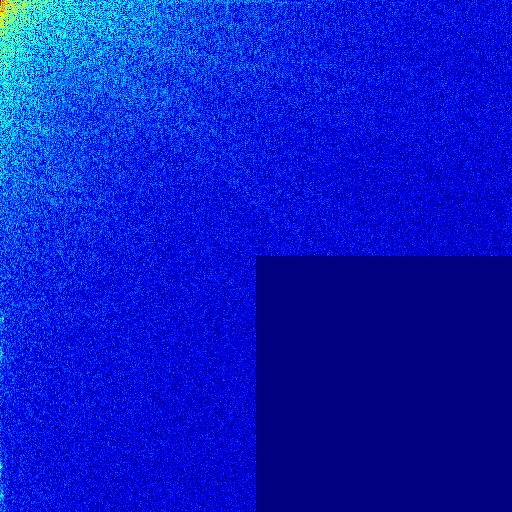
\includegraphics[scale=0.25]{../ImageRes/dct_masked0_1.jpg} 
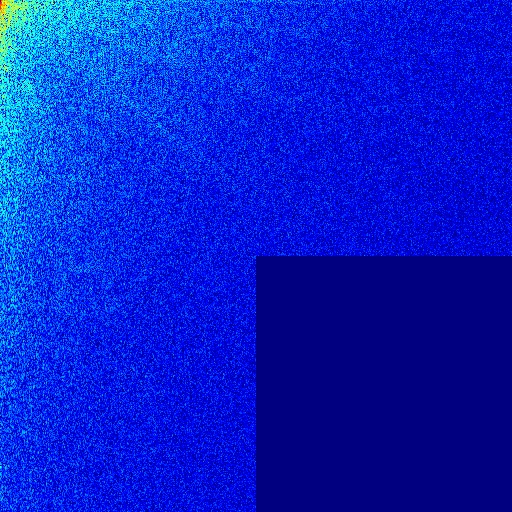
\includegraphics[scale=0.25]{../ImageRes/dct_masked0_2.jpg} 
\caption{Coefficients DCT pour les canaux Y, Cb et Cr de l'image "boats.pgm" après masquage coin bas droit}
\end{center}
\end{figure}

\begin{figure}[H]
\begin{center}

\includegraphics[scale=0.25]{../ImageRes/dct_masked0_histo_0.jpg} 

\includegraphics[scale=0.25]{../ImageRes/dct_masked0_histo_1.jpg} 
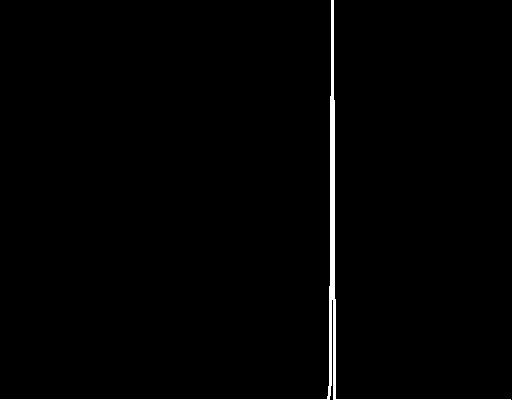
\includegraphics[scale=0.25]{../ImageRes/dct_masked0_histo_2.jpg} 
\caption{Histogrammes des coefficients DCT pour les canaux Y, Cb et Cr de l'image "boats.pgm" après masquage coin bas droit}
\end{center}
\end{figure}

\begin{itemize}
\item Entropie canal Y : 4.26638
\item Entropie canal Cr : 2.40643
\item Entropie canal Cb : 2.63162
\end{itemize}

\begin{figure}[H]
\begin{center}
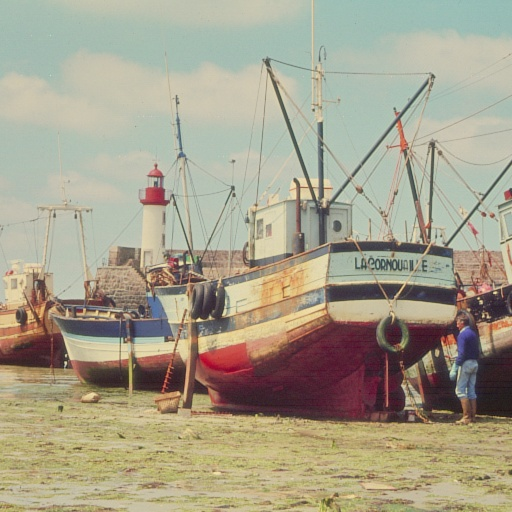
\includegraphics[scale=0.4]{../ImageRes/idct_masked0_result.jpg} 

\includegraphics[scale=0.4]{../ImageRes/idct_masked0_disto.jpg} 
\caption{Résultat de la DCT inverse et carte de distortion après masquage coin bas droit}
\end{center}
\end{figure}

\begin{itemize}
\item EQM : 4.49392
\item PSNR : 41.6045
\end{itemize}

\subsubsection{Deuxième masquage : moitié droite}


\begin{figure}[H]
\begin{center}
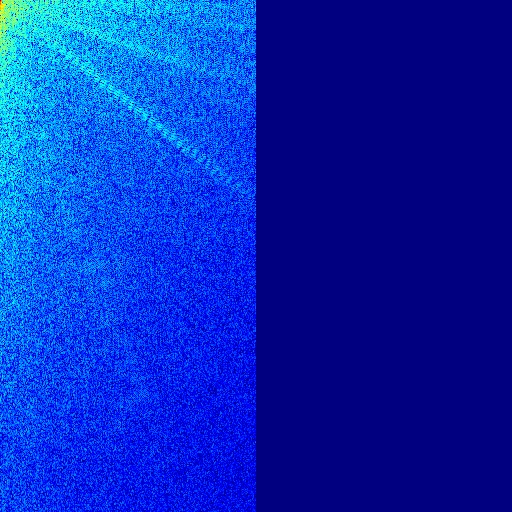
\includegraphics[scale=0.25]{../ImageRes/dct_masked1_0.jpg} 
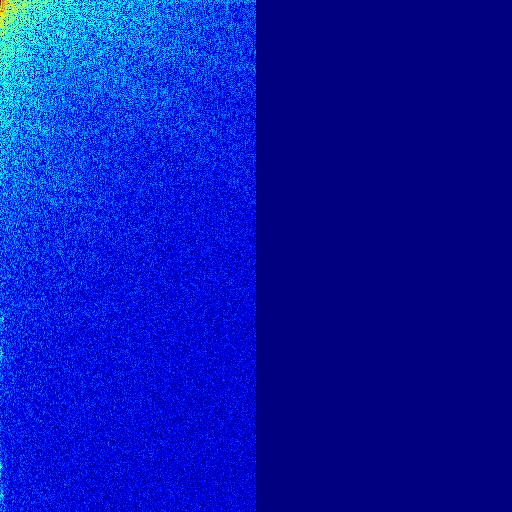
\includegraphics[scale=0.25]{../ImageRes/dct_masked1_1.jpg} 
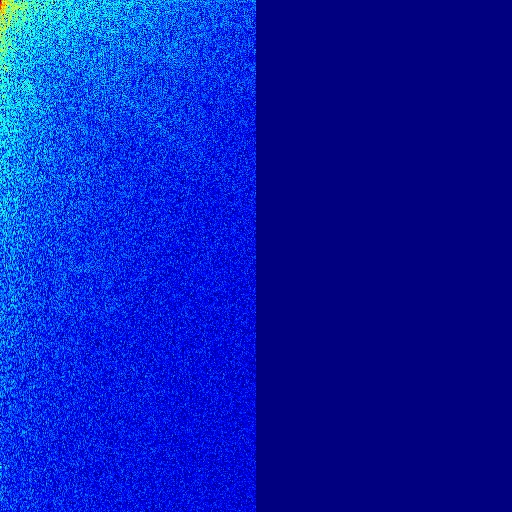
\includegraphics[scale=0.25]{../ImageRes/dct_masked1_2.jpg} 
\caption{Coefficients DCT pour les canaux Y, Cb et Cr de l'image "boats.pgm" après masquage moitié droite}
\end{center}
\end{figure}

\begin{figure}[H]
\begin{center}

\includegraphics[scale=0.25]{../ImageRes/dct_masked1_histo_0.jpg} 

\includegraphics[scale=0.25]{../ImageRes/dct_masked1_histo_1.jpg} 
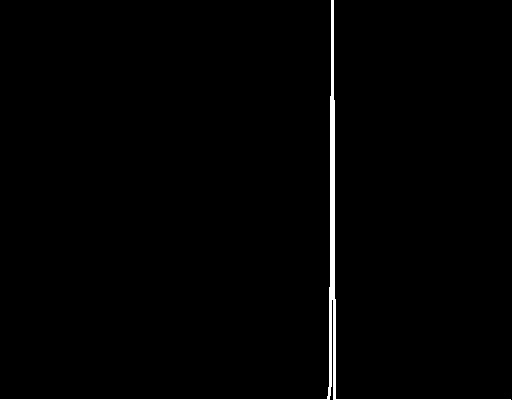
\includegraphics[scale=0.25]{../ImageRes/dct_masked1_histo_2.jpg} 
\caption{Histogrammes des coefficients DCT pour les canaux Y, Cb et Cr de l'image "boats.pgm" après masquage moitié droite}
\end{center}
\end{figure}

\begin{itemize}
\item Entropie canal Y : 3.41211
\item Entropie canal Cr : 2.03295
\item Entropie canal Cb : 2.25182
\end{itemize}

\begin{figure}[H]
\begin{center}
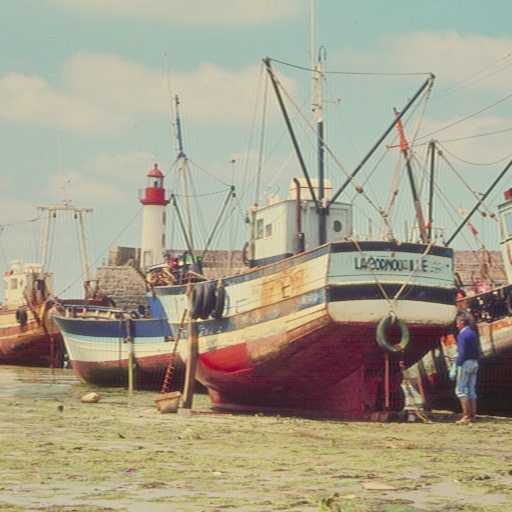
\includegraphics[scale=0.4]{../ImageRes/idct_masked1_result.jpg} 

\includegraphics[scale=0.4]{../ImageRes/idct_masked1_disto.jpg} 
\caption{Résultat de la DCT inverse et carte de distortion après masquage moitié droite}
\end{center}
\end{figure}

\begin{itemize}
\item EQM : 23.6301
\item PSNR : 34.3962
\end{itemize}

\subsubsection{Troisième masquage : moitié bas}

\begin{figure}[H]
\begin{center}
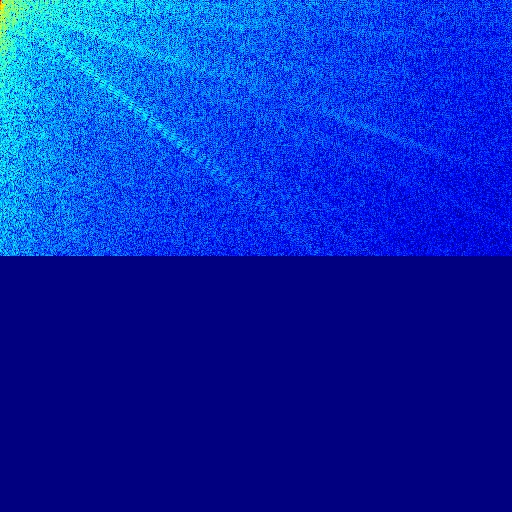
\includegraphics[scale=0.25]{../ImageRes/dct_masked2_0.jpg} 
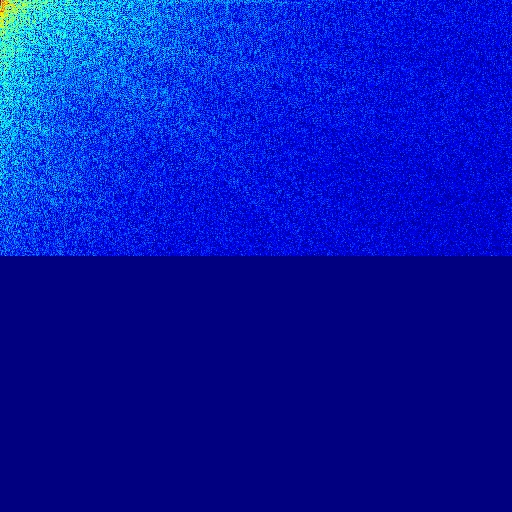
\includegraphics[scale=0.25]{../ImageRes/dct_masked2_1.jpg} 
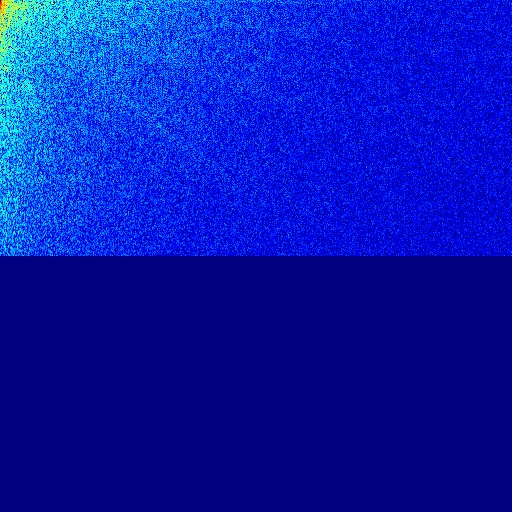
\includegraphics[scale=0.25]{../ImageRes/dct_masked2_2.jpg} 
\caption{Coefficients DCT pour les canaux Y, Cb et Cr de l'image "boats.pgm" après masquage moitié bas}
\end{center}
\end{figure}

\begin{figure}[H]
\begin{center}

\includegraphics[scale=0.25]{../ImageRes/dct_masked2_histo_0.jpg} 

\includegraphics[scale=0.25]{../ImageRes/dct_masked2_histo_1.jpg} 
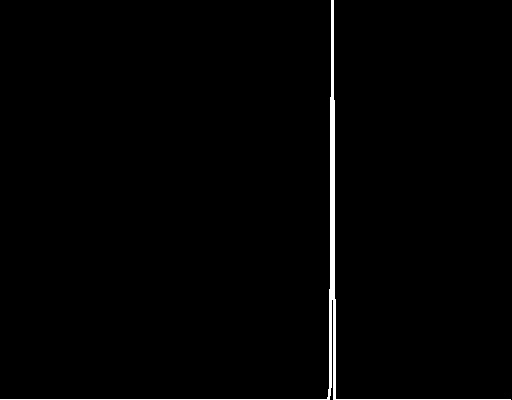
\includegraphics[scale=0.25]{../ImageRes/dct_masked2_histo_2.jpg} 
\caption{Histogrammes des coefficients DCT pour les canaux Y, Cb et Cr de l'image "boats.pgm" après masquage moitié bas}
\end{center}
\end{figure}

\begin{itemize}
\item Entropie canal Y : 3.40015
\item Entropie canal Cr : 2.04095
\item Entropie canal Cb : 2.13661
\end{itemize}

\begin{figure}[H]
\begin{center}
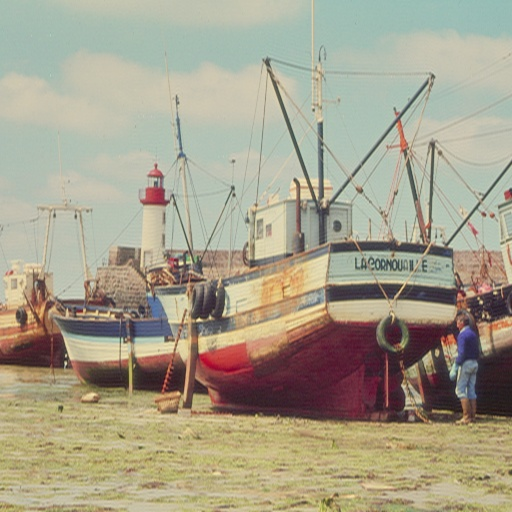
\includegraphics[scale=0.4]{../ImageRes/idct_masked2_result.jpg} 

\includegraphics[scale=0.4]{../ImageRes/idct_masked2_disto.jpg} 
\caption{Résultat de la DCT inverse et carte de distortion après masquage moitié bas}
\end{center}
\end{figure}

\begin{itemize}
\item EQM : 28.9478
\item PSNR : 33.5147
\end{itemize}

\subsubsection{Quatrième masquage : coin bas gauche}

\begin{figure}[H]
\begin{center}
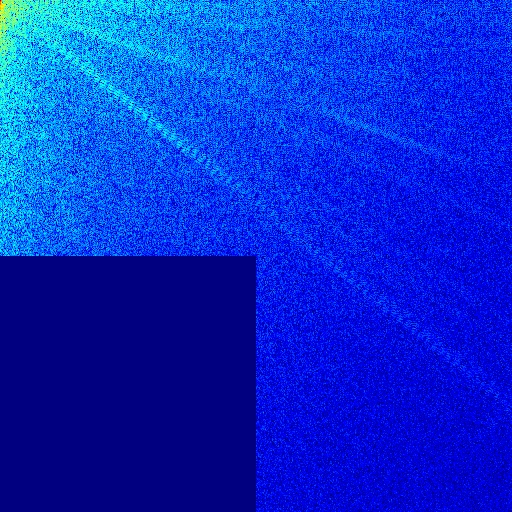
\includegraphics[scale=0.25]{../ImageRes/dct_masked3_0.jpg} 
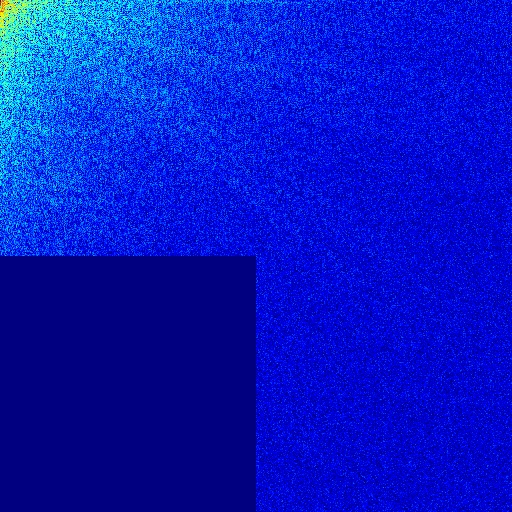
\includegraphics[scale=0.25]{../ImageRes/dct_masked3_1.jpg} 
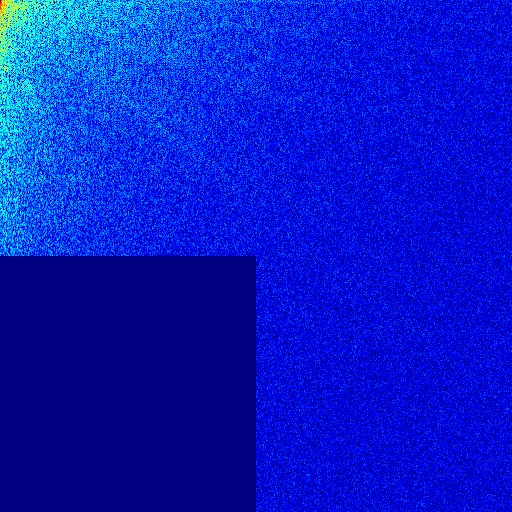
\includegraphics[scale=0.25]{../ImageRes/dct_masked3_2.jpg} 
\caption{Coefficients DCT pour les canaux Y, Cb et Cr de l'image "boats.pgm" après masquage coin bas gauche}
\end{center}
\end{figure}

\begin{figure}[H]
\begin{center}

\includegraphics[scale=0.25]{../ImageRes/dct_masked3_histo_0.jpg} 

\includegraphics[scale=0.25]{../ImageRes/dct_masked3_histo_1.jpg} 
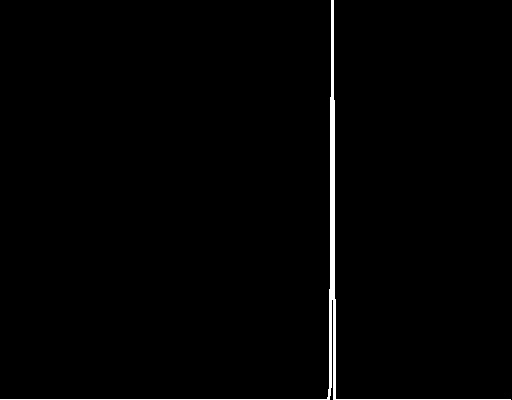
\includegraphics[scale=0.25]{../ImageRes/dct_masked3_histo_2.jpg} 
\caption{Histogrammes des coefficients DCT pour les canaux Y, Cb et Cr de l'image "boats.pgm" après masquage coin bas gauche}
\end{center}
\end{figure}

\begin{itemize}
\item Entropie canal Y : 3.98762
\item Entropie canal Cr : 2.28932
\item Entropie canal Cb : 2.44441
\end{itemize}

\begin{figure}[H]
\begin{center}
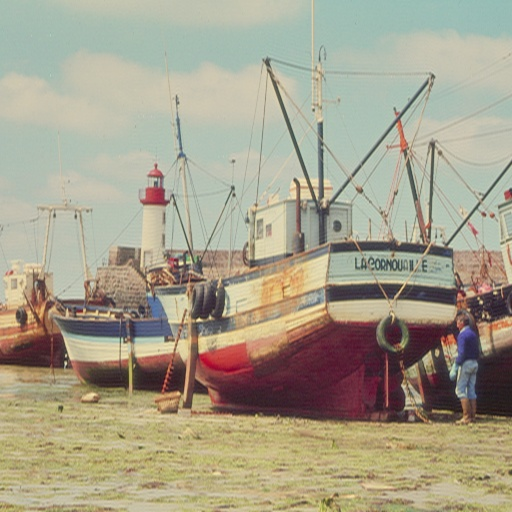
\includegraphics[scale=0.4]{../ImageRes/idct_masked2_result.jpg} 

\includegraphics[scale=0.4]{../ImageRes/idct_masked2_disto.jpg} 
\caption{Résultat de la DCT inverse et carte de distortion après masquage coin bas gauche}
\end{center}
\end{figure}

\begin{itemize}
\item EQM : 24.5393
\item PSNR : 34.2322
\end{itemize}

\subsubsection{Interprétations}
Expliquer les résultats observés.
Sommes nous dans un contexte de transformation globale ?

\subsection{Etude de la DCT appliquée par bloc 8x8}
Nous avons commencé par mettre en place la DCT par bloc 8x8 et la DCT inverse. Nous observons les résultats suivant :

\begin{figure}[H]
\begin{center}
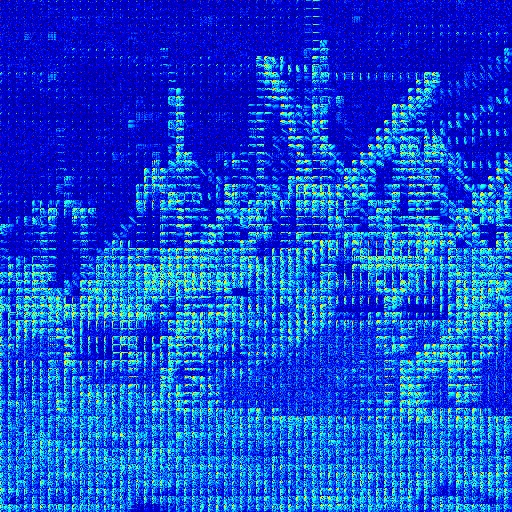
\includegraphics[scale=0.25]{../ImageRes/blockdct_0.jpg} 
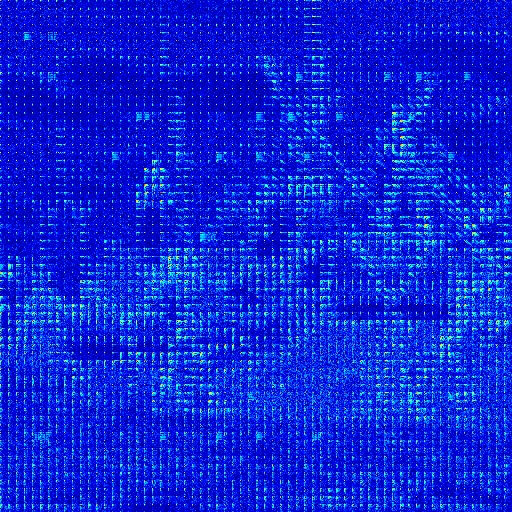
\includegraphics[scale=0.25]{../ImageRes/blockdct_1.jpg} 
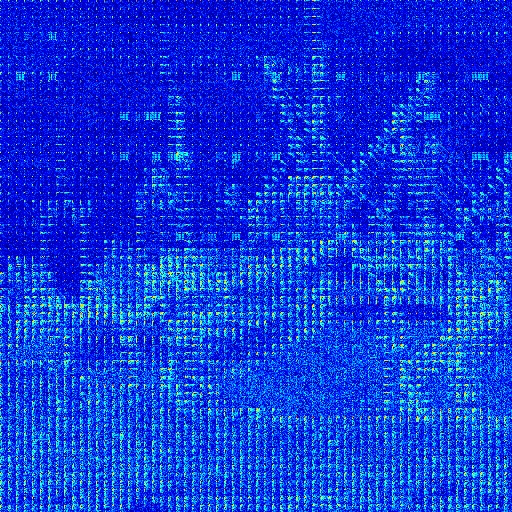
\includegraphics[scale=0.25]{../ImageRes/blockdct_2.jpg} 
\caption{Coefficients DCT par blocs 8x8 pour les canaux Y, Cb et Cr de l'image "boats.pgm"}
\end{center}
\end{figure}

\begin{figure}[H]
\begin{center}
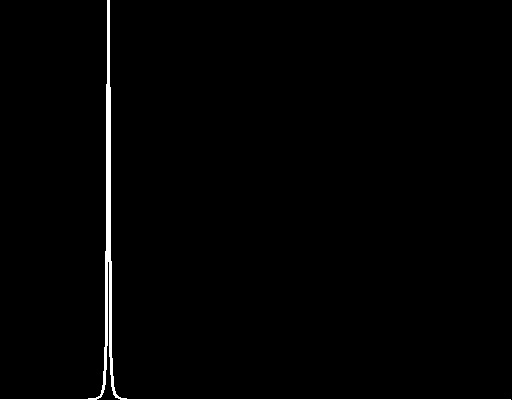
\includegraphics[scale=0.25]{../ImageRes/blockdct_histo_0.jpg} 
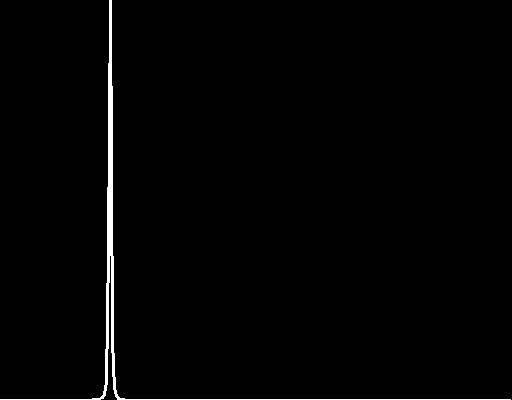
\includegraphics[scale=0.25]{../ImageRes/blockdct_histo_1.jpg} 
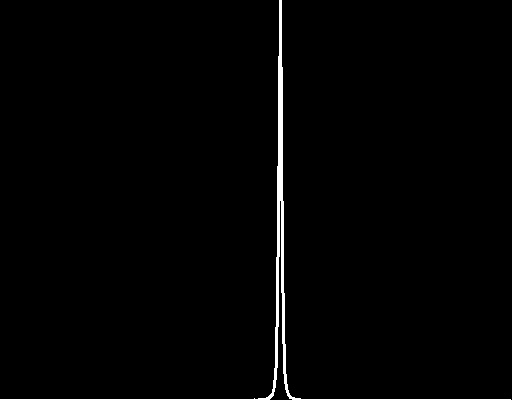
\includegraphics[scale=0.25]{../ImageRes/blockdct_histo_2.jpg} 
\caption{Histogrammes des coefficients DCT par blocs 8x8 pour les canaux Y, Cb et Cr de l'image "boats.pgm"}
\end{center}
\end{figure}

\begin{itemize}
\item Entropie canal Y : 3.7306
\item Entropie canal Cr : 2.38546
\item Entropie canal Cb : 2.63086
\end{itemize}

\begin{figure}[H]
\begin{center}
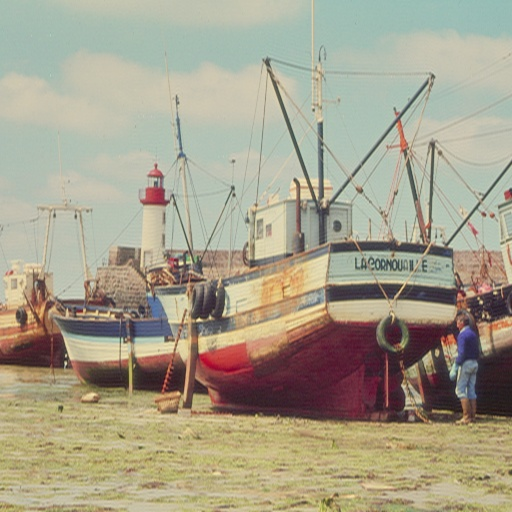
\includegraphics[scale=0.5]{../ImageRes/idct_masked2_result.jpg} 
\caption{Résultat de la DCT par blocs 8x8 inverse}
\end{center}
\end{figure}

\begin{itemize}
\item EQM : 0
\item PSNR : inf
\end{itemize}

Ces résultats confirment le bon fonctionnement de notre transformée.

\subsubsection{Annulation de coefficients de la DCT par bloc 8x8}

\begin{figure}[H]
\begin{center}
\includegraphics[scale=0.25]{../ImageRes/blockdct_masked_0.jpg} 
\includegraphics[scale=0.25]{../ImageRes/blockdct_masked_1.jpg} 
\includegraphics[scale=0.25]{../ImageRes/blockdct_masked_2.jpg} 
\caption{Coefficients DCT par blocs 8x8 pour les canaux Y, Cb et Cr de l'image "boats.pgm" après masquage}
\end{center}
\end{figure}

\begin{figure}[H]
\begin{center}
\includegraphics[scale=0.25]{../ImageRes/blockdct_masked_histo_0.jpg} 
\includegraphics[scale=0.25]{../ImageRes/blockdct_masked_histo_1.jpg} 
\includegraphics[scale=0.25]{../ImageRes/blockdct_masked_histo_2.jpg} 
\caption{Histogrammes des coefficients DCT par blocs 8x8 pour les canaux Y, Cb et Cr de l'image "boats.pgm" après masquage}
\end{center}
\end{figure}

\begin{itemize}
\item Entropie canal Y : 1.62577
\item Entropie canal Cr : 1.30891
\item Entropie canal Cb : 1.36591
\end{itemize}

\begin{figure}[H]
\begin{center}
\includegraphics[scale=0.4]{../ImageRes/blockidct_masked_result.jpg} 
\includegraphics[scale=0.4]{../ImageRes/blockidct_masked_disto.jpg} 
\caption{Résultat de la DCT par blocs 8x8 inverse et carte de distortion après masquage}
\end{center}
\end{figure}

\begin{itemize}
\item EQM : 49.7125
\item PSNR : 31.1661
\end{itemize}

\subsubsection{Application d'une transformation aux coefficients de la DCT par bloc 8x8}

\begin{figure}[H]
\begin{center}
\includegraphics[scale=0.25]{../ImageRes/blockdct_transform_0.jpg} 
\includegraphics[scale=0.25]{../ImageRes/blockdct_transform_1.jpg} 
\includegraphics[scale=0.25]{../ImageRes/blockdct_transform_2.jpg} 
\caption{Coefficients DCT par blocs 8x8 pour les canaux Y, Cb et Cr de l'image "boats.pgm" après transformation}
\end{center}
\end{figure}

\begin{figure}[H]
\begin{center}
\includegraphics[scale=0.25]{../ImageRes/blockdct_transform_histo_0.jpg} 
\includegraphics[scale=0.25]{../ImageRes/blockdct_transform_histo_1.jpg} 
\includegraphics[scale=0.25]{../ImageRes/blockdct_transform_histo_2.jpg} 
\caption{Histogrammes des coefficients DCT par blocs 8x8 pour les canaux Y, Cb et Cr de l'image "boats.pgm" après transformation}
\end{center}
\end{figure}

\begin{itemize}
\item Entropie canal Y : 0.995572
\item Entropie canal Cr : 0.380482
\item Entropie canal Cb : 0.422024
\end{itemize}

\begin{figure}[H]
\begin{center}
\includegraphics[scale=0.4]{../ImageRes/blockidct_transform_result.jpg} 
\includegraphics[scale=0.4]{../ImageRes/blockidct_transform_disto.jpg} 
\caption{Résultat de la DCT par blocs 8x8 inverse et carte de distortion après transformation}
\end{center}
\end{figure}

\begin{itemize}
\item EQM : 43.8357
\item PSNR : 31.7125
\end{itemize}

\section{Conclusion}


\begin{comment}

%Commande pour le sommaire

\renewcommand{\contentsname}{\large Sommaire} % Change le nom en sommaire
\setcounter{tocdepth}{2} % Défini la profondeur d'une table des matières
\tableofcontents
\newpage

\end{comment}

\newpage


%Commande pour le sommaire des figures

\renewcommand*\listfigurename{\large Liste des figures}
\listoffigures
\newpage


\end{document}
